% !TeX root = ../main.tex
% Add the above to each chapter to make compiling the PDF easier in some editors.

\chapter{Introduction}\label{chapter:introduction}

It is safe to say that the internet paved the way for many things for humanity.
Media such as images, video and audio can be shared across websites and applications, knowledge can be stored in faraway servers and retrieved with ease in text format using mobile devices, and products and services can be bought with the click of a button or a tap on a screen.
Interactions, media and information make up for massive amounts of data that flow through complex computer systems, which in turn generate even more data and information.

Researchers have found ways to leverage the magnitude of data that is being produced every second by countless systems all around the world.
One of the most recent and most popular uses of this huge variety and quantity of data is machine learning (ML).
Machine learning can be defined as a set of techniques that use data to improve performance in a set of tasks.
Today, for example, we feed data to machine learning models to calculate what is the probability that a webpage visitor will buy certain products, or the chances that it is going to rain in a few days or to generate elaborate text and stunning, never-before-seen pictures.

Recently, models such as BERT \cite{devlin2018bert}, DALL-E \cite{ramesh2021zero}, GPT-3 \cite{brown2020gpt3} and others have become incredibly popular thanks to their outstanding results and endless possibilities.
DALL-E for example can generate high-quality realistic images and art starting from a text description written in natural language.
These models however require massive amounts of data as well as very expensive computational resources, such as graphical processing units and tensor processing units (TPUs).
In recent years, the size of neural network models has been steadily increasing exponentially, as shown by \autoref{fig:model-size-over-time}.
A simple calculation shows that the neural network model Megatron-Turing-NLG 530B \cite{smith2022megatronturingnlg} would take roughly $530 \times 4 = 2120\texttt{GB}$ of memory to simply hold its 530 billion weights.

Furthermore, training a neural network model requires even more memory.
Intermediate computation outputs such as gradient and optimizer states sometimes require 2 or 3 times as much memory than just the model parameters, making GPU memory one of the main bottlenecks in training huge neural network models.
While some of these issues can be tackled using clever techniques such as parameter quantization, pruning and compression, they must not be considered one-fits-all solutions.
Some models are simply too big to be trained on a single device.
This problem is exacerbated by factors such as GPU prices and much slower growth of their memory size.
\autoref{fig:gpu-vram-over-time} shows how GPU memory has been increasing from 2016 to 2022.

\begin{figure}[h]
    \caption{GPU VRAM over the past 4 years. The growth is mostly linear, doubling }
    \label{fig:gpu-vram-over-time}
    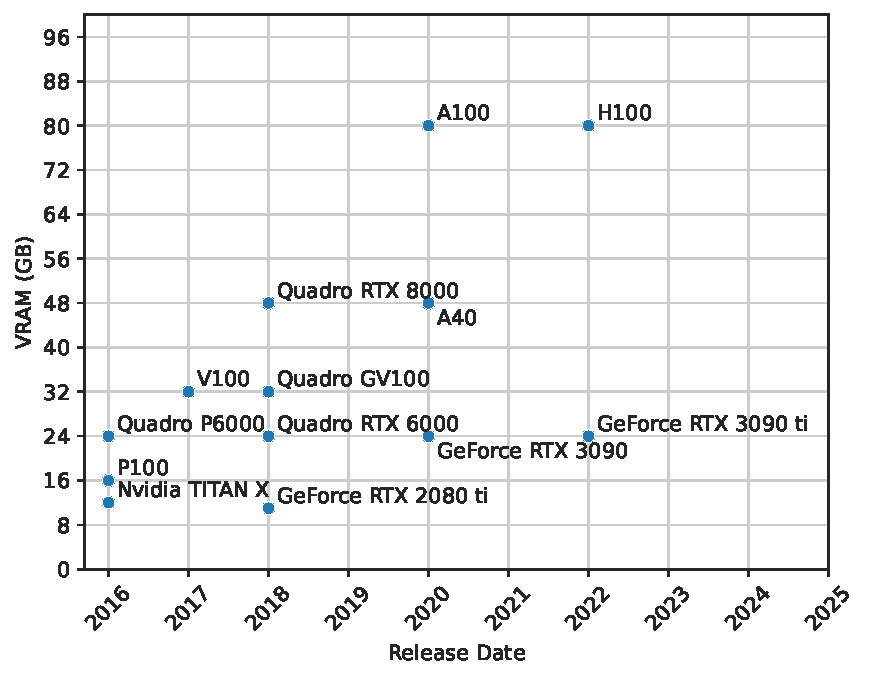
\includegraphics[width=\textwidth]{./figures/gpu-vram-over-time.pdf}
\end{figure}

\begin{figure}[h]
    \caption{Model size over the past 4 years: ELMo \cite{peters2018elmo}, BERT \cite{devlin2018bert}, GPT-2 \cite{radford2019language}, Megatron-LM \cite{shoeybi2019megatronlm}, T-5 \cite{raffael2019t5}, Turing-NLG \cite{microsoft2020turingnlg}, GPT-3 \cite{brown2020gpt3}, Megatron-Turing-NLG \cite{smith2022megatronturingnlg}}
    \label{fig:model-size-over-time}
    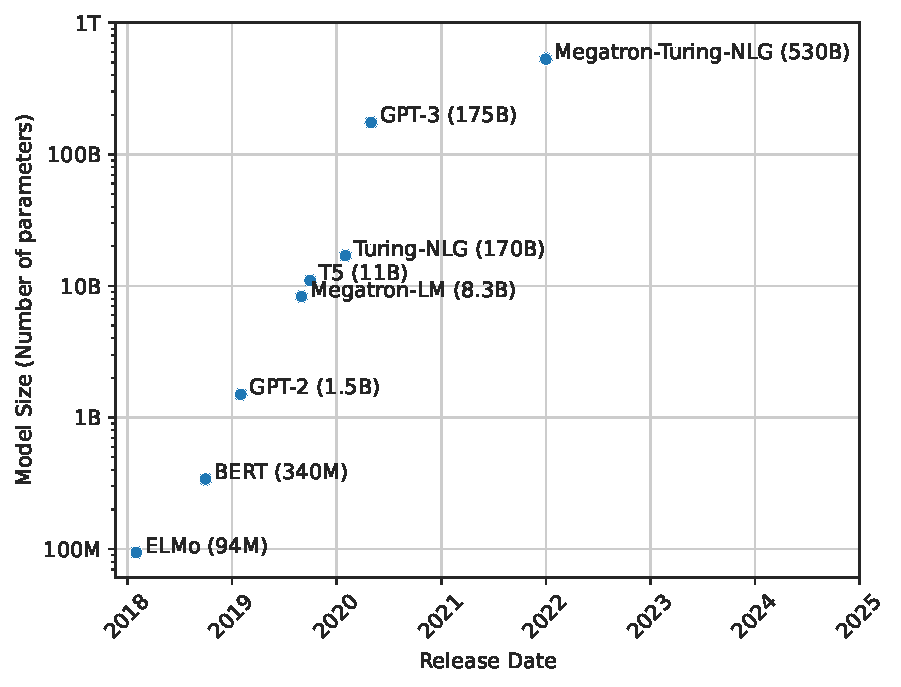
\includegraphics[width=\textwidth]{./figures/model-size-over-time.pdf}
\end{figure}

The characteristics of the latest GPU released by NVIDIA earlier in 2022, the H100 with 80GB of memory, an amount that hasn't changed since its direct predecessor A100.

To tackle this problem, practitioners studied and developed distributed computing techniques to train models that do not fit entirely in a single GPU's memory, distributing the training load to potentially thousands of devices.

These techniques can be briefly categorized as follows:
\begin{itemize}
    \item \textit{Data parallelism}. Given a set of $n$ devices, an instance of the model is trained on each one of the devices. Usually, gradients obtained during backpropagation are then aggregated across all the devices using techniques such as \textit{AllReduce}. This technique however does not work very well with models that exceed a single device's available memory and is therefore used in applications with low-memory devices such as \textit{Federated Learning} \cite{li2019federatedlearning}.

    \item \textit{Model parallelism}. A deep neural network is conceptually split into $n$ partitions across $n$ devices, each hosting a different partition and set of weights. An early notable example of model parallelism is AlexNet \cite{alexnet2012}, where the authors decided to split the computation of some of the layers across two GPUs with 3GB of ram each, a concept illustrated in \autoref{fig:alexnet}. This technique relieves the burden of a single node to host all of the weights of a model but is also more sensitive to issues with communication across nodes.

    \item \textit{Pipeline parallelism}. A combination between model parallelism and data parallelism. Introduced by \cite{huang2018gpipe}, pipeline parallelism consists in splitting a batch into micro-batches across the available computing devices, leading to fewer dead wait times.
    \item \textit{Tensor parallelism}. Tensor operations for huge neural network models can become a bottleneck, as they can require more memory than the host's device can handle and can become slow in general. Tensor parallelism can alleviate a single node's computational burden by splitting a tensor operation across many devices. This technique has been first introduced in neural network models in \cite{dean2012distbelief} with a framework called DistBelief.
    \item \textit{Mixture-of-Experts}. Instead of conceptually splitting a model, we construct multiple, different models. Each of them specializes in a different subset of the complete set of training cases, helped by a gating function. This has been first introduced in 1991 by \cite{Jacobs1991mixtureofexperts} but has recently gained traction due to its attractiveness in numerous tasks.
\end{itemize}

\begin{figure}[h]
    \caption{AlexNet \cite{alexnet2012} architecture shows one of the first examples of model parallelism. The training of convolutional layers is split across two GPUs, as the size of the model during training exceeded the available memory of a single GPU.}
    \label{fig:alexnet}
    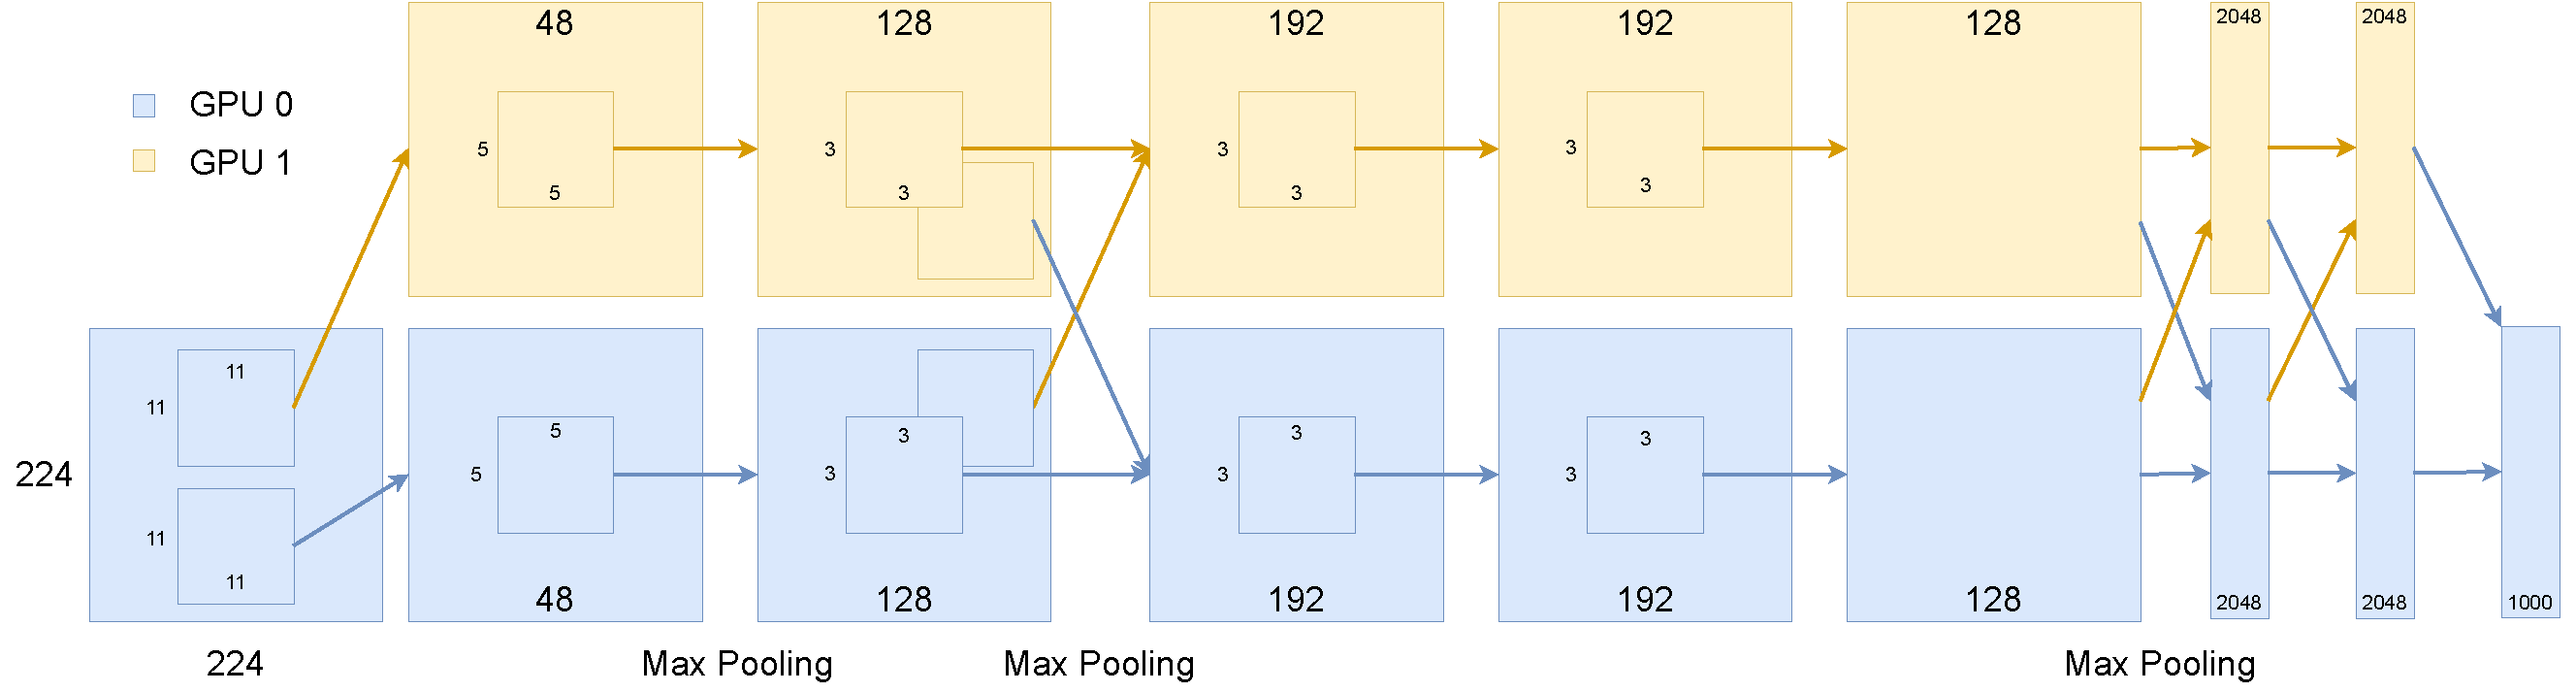
\includegraphics[width=\textwidth]{./figures/alexnet.pdf}
\end{figure}

\section{Motivation}

Most of the frameworks and papers built on top of the techniques presented previously approach scalability issues by employing tremendous amounts of expensive, top-of-the-art and heterogeneous hardware.
However, universities, small companies and hobbyists that want to train the models described in these papers do not necessarily have access to a such vast amount of resources, limiting possibilities and research directions.

The framework Hivemind \cite{riabinin2020hivemind} aims to help with these issues by allowing distributed neural network training across the internet using heterogeneous devices.
The authors provide two types of training: \textit{decentralized parameter averaging} and \textit{decentralized mixture-of-experts}.

Hivemind implements two training algorithms: ``Decentralized Mixture-of-Experts'' (DMoE) \cite{ryabinin2020learning} and ``Parameter Averaging''.
DMoE has been shown to work well for decentralized deep neural network training using large amounts of consumer-grade hardware.
The algorithm described in the original paper employs a combination of decentralized and Mixture-of-Experts \cite{shazeer2017outrageously} techniques.
This allows thousands of computing devices to join forces and train a single neural network model together.

DMoE achieves these results by splitting the target neural network model into different parts called partitions, similarly to model parallelism.
Each partition is then replicated across a subset of workers participating in the training.
Next, a gating function is used to select which workers can perform the next operation on the given input.
After the workers have been selected and located using a Distributed Hash Table (DHT), the input data is sent to the workers, and a forward pass is performed.
A similar algorithm is applied during the backward pass.
DMoE proved that scaling model training to thousands of heterogeneous compute nodes is possible, thus enabling large-scale community research projects.

% NOTE: for now we keep it here
% Although DMoE is robust against training latency, it also requires large amounts of data to be exchanged between every participant worker.
% However, most participants that join the training network do not have datacenter-grade network connections and bandwidth.
% Therefore, the communications needed to perform training may saturate a worker's network.
% An approach suggested by \cite{ryabinin2020learning} to reduce the network load is to compress and convert tensors to a lower precision before transfer.

Despite an academic interest in DMoE, we have eventually decided against performing any experimentation on DMoE for this thesis, as the API was not stable enough at the time of experiments.
For this reason, the focus of this thesis is on decentralized parameter averaging, the second type of training algorithm implemented by Hivemind.
With decentralized parameter averaging, each node participating in the training must have a copy of the model in memory.
Every node performs training at its own pace, accumulating samples toward a global goal called ``target batch size''.
Once this goal has been reached, an averaging round starts.
The final gradients are calculated depending on the contribution in terms of the number of samples done by each peer, ensuring stability in case of peer failure.

Decentralized parameter averaging has shown promising results \cite{learning30:online}, successfully training a modified version of DALL-E using 40 peers over two months.
TODO: add something else about this.

Over the last few years, research and software libraries like Hivemind have been focused on reducing and optimizing deep neural network model training times with techniques such as data and model parallelism.
In \cite{xin2021production} however, the authors show that as much as 45\% of total training time may be spent on preprocessing tasks alone.
Despite this, the impact of preprocessing pipelines is often ignored in current research.
As noted by \citeauthor{isenko2022bottleneck} \cite{isenko2022bottleneck}, it is crucial to find and analyze bottlenecks during computation to maximize performance.
In their work, they also detail several possible improvements that can be applied in preprocessing pipelines, increasing throughput under certain circumstances.
Intuitively, given the high amount of communications and data loading needed by parameter averaging, training may be subject to inefficiencies.
Using the techniques and findings showcased in \cite{isenko2022bottleneck}, this thesis further aims to find bottlenecks while training with Hivemind.

\section{Approach}

In this thesis, we will compare regular training using a single node with 16vCPUs to training using Hivemind with multiple peers, where the sum of vCPUs per peer always amounts to 16.
Also, the number of samples 
We compare training with key Hivemind settings, namely:
\begin{itemize}
    \item Batch size;
    \item Learning rate;
    \item Number of peers involved in the training;
    \item Target number of samples that must be globally reached by all peers to perform an averaging round;
    \item Applying the gradients at every step or accumulating them until the next averaging round.
\end{itemize}

As we test the software and its limitations, we might find possible areas of improvement in Hivemind.
Whenever possible, we will further contribute using the knowledge gathered through our experiments by improving the Hivemind \cite{hivemind} source code.

\section{Contributions}

Our contributions are as follows:
\begin{itemize}
    \item We analyze the challenges of optimizing preprocessing pipelines in decentralized distributed training and provide insights on possible improvements
    \item We verify the effectiveness of Hivemind for different peer hardware configurations concerning preprocessing pipelines
    \item We use the gained knowledge and insights to contribute to the Hivemind open-source library.
\end{itemize}
